

\setchapterpreamble[c][.7\textwidth]{\itshape\dgrau\small
    In diesem Vortrag werden Grudbausteine der Analysis, wie Ungleichungen, Abstand, Umgebungen und Folgenkonvergenz, besprochen und mit Beispielen illustriert. Die Intuitionsbildung soll hier Vorrang vor Rigorosität haben.
\vspace{24pt}}


\chapter{Ausblick auf die Analysis}


\section{Mehr über reelle Zahlen}


\begin{bem}[Buchtipp]
    In diesem Vortrag soll ein Überblick über einige wichtige Konzepte der Analysis gegeben werden. Am wichtigsten ist mir hier die Konstruktion von Bildern und intuitiven Erklärungen, weshalb vergleichsweise viele Aussagen nicht bewiesen, sondern nur mit einer Erklärung plausibilisiert werden.
    
    Möchtest du es genau wissen, lege ich dir das Analysis-Lehrbuch \cite{AE06} ans Herz, mit dem auch ich als Erstsemester den Analysis-Stoff gelernt habe und das selbst nach sechs Jahren Studium zu den besten Mathe-Lehrbüchern gehört, die ich gelesen habe. Einige wenige Kritikpunkte sind für mich ihre eigenwillige Notation, die das Buch ungeeignet zum schnellen Nachschlagen macht, sowie die nachlassende Qualität der nachfolgenden Bände zu Ana2 und Ana3. Über den Link im Literaturverzeichnis kannst du dir das Buch kostenlos aus dem Uni-Netz herunterladen. Wirf mal einen Blick hinein und schau, ob es dich anspricht!
\end{bem}


\begin{bem}[Struktur auf $\R$]
    Sowohl die rationalen Zahlen $\Q$ als auch die reellen Zahlen $\R$ bilden einen sogenannten „angeordneten Körper“. Die genaue Definition dieses Begriffs führte zu weit über diesen Vortrag hinaus. In etwa heißt es folgendermaßen:
    \begin{itemize}
        \item Mit reellen bzw. rationalen Zahlen lässt sich rechnen. Sie lassen sich addieren, subtrahieren, multiplizieren und, mit Ausnahme der Zahl $0$, auch dividieren. Dieser algebraische Aspekt wurde im Kapitel über Verknüpfungen vertieft.
        \item $(\R,\le)$ und $(\Q,\le)$ sind totalgeordnete Mengen, d.h. reelle bzw. rationale Zahlen können hinsichtlich ihrer „Größe“ miteinander verglichen werden. Dieser Aspekt wurde im Kapitel über Relationen vertieft.
        \item Die Ordnungen auf $\R$ und $\Q$ sind mit den arithmetischen Operationen verwoben, d.h. beide Strukturen existieren nicht völlig getrennt voneinander, sondern hängen auf gewisse Weise miteinander zusammen. Diese „Verträglichkeit“ wird im folgenden Satz explizit gemacht:
    \end{itemize}
\end{bem}


\begin{satz}[Einige Rechenregeln für Ungleichungen] \label{ungleichungregeln}
    Für alle reellen Zahlen $x,y,a,\lambda\in \R$ gilt:
    \begingroup
    \allowdisplaybreaks
    \begin{alignat*}{4}
        x&\le y &\qquad&\iff&\qquad x+a&\le y+a \\
        x&\le y &\qquad&\iff&\qquad x-a&\le y-a \\
        x&\le y &\qquad&\iff&\qquad \lambda \cdot x&\le \lambda \cdot y &\qquad&\qquad (\textnormal{sofern $\lambda>0$}) \\[0.5em]
        x&\le y &\qquad&\iff&\qquad \frac{x}{\lambda} &\le \frac{y}{\lambda} &\qquad&\qquad (\textnormal{sofern $\lambda>0$}) \\[0.5em]
        x&\le y &\qquad&\iff&\qquad \lambda \cdot y&\le \lambda \cdot x &\qquad&\qquad (\textnormal{sofern $\lambda<0$}) \\[0.5em]
        x&\le y &\qquad&\iff&\qquad \frac{y}{\lambda} &\le \frac{x}{\lambda} &\qquad&\qquad (\textnormal{sofern $\lambda<0$}) \\[0.5em]
        x&\le y &\qquad &\iff&\qquad -y&\le -x \\[0.5em]
        x&\le y &\qquad&\iff&\qquad \frac{1}{y} & \le\frac{1}{x} &\qquad&\qquad (\textnormal{sofern $x,y>0$})
    \end{alignat*}
    \endgroup
    Alle diese Regeln gelten auch, wenn man überall die kleinergleich-Relation $\le$ durch die strikt-kleiner-Relation $<$ ersetzt.
\end{satz}


\begin{bem} \label{ungleichungerklaerung}
    Einige dieser Regeln werden gelegentlich als „Anordnungsaxiome“ bezeichnet. Ich werde hier auf einen Beweis verzichten\footnote{Beweise findest du z.B. in \cite{AE06}, Satz I.8.9.}.
    \begin{itemize}
        \item Die ersten beiden Regeln besagen, dass Addition und Subtraktion jeweils Äquivalenz\-umformungen für Ungleichungen darstellen. Man sagt auch, die Ordnungsrelation sei \emph{translationsinvariant}, weil sich Addition bzw. Subtraktion als „Verschiebung“ der Zahlengerade vorstellen lassen.
        \item Die nächsten beiden Regeln besagen, dass auch Multiplikation und Division jeweils Äquivalenzumformungen sind, sofern sie mit einer \emph{positiven} Zahl geschehen.
        \item Bei Multiplikation und Division mit einer negativen Zahl handelt es sich um „Anti-Äquivalenzumformungen“: bei solchen Umformungen muss die Ungleichung umgedreht werden. Ebenso verhält es sich beim Vorzeichenwechsel und beim Bilden von Kehrwerten positiver Zahlen.
    \end{itemize}
\end{bem}


\begin{bsp} \label{bsp:ungleichungumstellen}
    Seien $n\in \N$ und $\varepsilon \in \R_{>0}$. Gegeben sei die folgende Ungleichung
        \[ \varepsilon > \frac{1}{n+1} \]
    die wir gerne nach der Zahl $n$ „umstellen“ würden.
    \begin{enumerate}
        \item Wegen $n\in \N$ ist $n+1$ eine positive Zahl, sodass beide Seiten der Ungleichung mit $n+1$ multipliziert werden können.
            \[ \varepsilon  > \frac{1}{n+1} \quad\iff\quad \varepsilon \cdot (n+1) > 1\]
        \item Da wir $\varepsilon>0$ vorausgesetzt haben, können beide Seiten der Ungleichung durch $\varepsilon$ dividiert werden:
            \[ \varepsilon \cdot (n+1) > 1 \quad\iff\quad n+1 > \frac{1}{\varepsilon} \]
        \item Schließlich können wir von beiden Seiten jeweils $1$ abziehen:
            \[ n+1 > \frac{1}{\varepsilon} \quad\iff\quad n > \frac{1}{\varepsilon}-1 \]
    \end{enumerate}
    Insgesamt haben wir damit die Ungleichung nach $n$ umgestellt:
        \[ \varepsilon > \frac{1}{n+1} \quad\iff\quad n > \frac{1}{\varepsilon}-1 \]
    Diese Umformungen werden später in die Beweisfindung für \cref{bsp:konvergenz} eingehen.
\end{bsp}


\begin{de}[* Die erweiterte Zahlengerade] \index{Erweiterte Zahlengerade}
    Gelegentlich ist es praktisch, die reellen Zahlen um zwei weitere Elemente „$\infty$“ und „$-\infty$“ zu erweitern. Das ist alles andere als mysteriös: wir fassen „$\infty$“ und „$-\infty$“ schlicht als „Symbole“ auf, als zwei weitere Elemente, die wir der Menge $\R$ künstlich hinzufügen. Die durch diese Hinzufügung entstehende Menge wird manchmal \textbf{erweiterte Zahlengerade} genannt und mit
        \[ \bar\R := \R\cup \{-\infty,\infty\} \]
    notiert. Um den beiden neuen Elementen $\pm \infty$ ihren intendierten Platz hinsichtlich der Ordnung von $\R$ zuzuweisen, legen wir fest, dass
        \begin{align*}
            -\infty \le  x \le \infty && (\text{für alle $x\in \bar \R$})
        \end{align*}
    d.h. „$-\infty$“ sei per Definition kleiner als jede reelle Zahl, „$\infty$“ dagegen größer als jede reelle Zahl. Es lässt sich zeigen, dass $(\bar \R,\le)$ auf diese Weise zu einer totalgeordneten Menge wird. Beachte, dass $\pm \infty$ keine reellen Zahlen sind und dass sich damit auch nur eingeschränkt rechnen lässt.
\end{de}


\begin{de}[Betrag und Signum] \index{Betrag} \index{Signum}
    Für eine reelle Zahl $a\in \R$ ist ihr \textbf{Betrag} definiert durch 
    \begin{align*}
        |a|:= \begin{cases}
            a&a\ge 0\\
            -a&a \le 0
        \end{cases}
    \end{align*}
    Ihr \textbf{Signum} (oder auch \textbf{Vorzeichen}) ist definiert durch:
    \begin{align*}
        \sgn(a) := \begin{cases}
            1 & a>0 \\
            0 & a=0 \\
            -1 & a<0
        \end{cases}
    \end{align*} 
    \begin{figure}[ht]
    \begin{minipage}{.48\textwidth}
        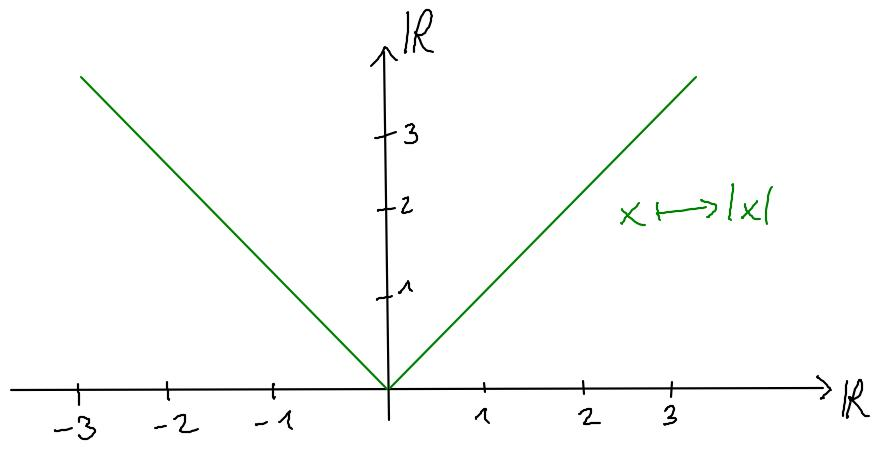
\includegraphics[width=7cm]{./_img/Betrag.jpeg}
        \centering \caption{Graph der Betragsfunktion.}
    \end{minipage}
    \quad
    \begin{minipage}{.48\textwidth}
        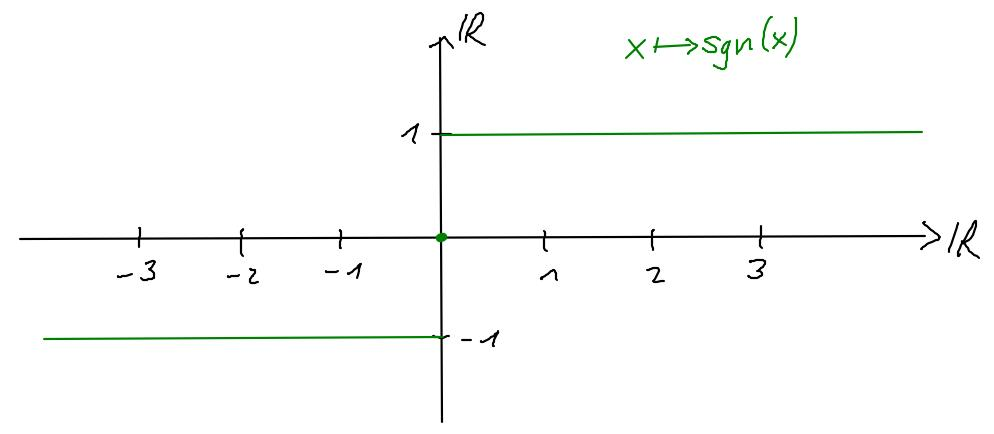
\includegraphics[width=7.5cm]{./_img/Signum.jpeg}
        \centering \caption{Graph der Signumsfunktion}
    \end{minipage}
    \end{figure}
\end{de}


\begin{bsp}
    Beispielsweise ist
    \begin{align*}
        \vert 3\vert &= 3 & \vert -7\vert &=7 & \vert 0\vert=0 \\
        \sgn(3) & = 1 & \sgn(-7) & = -1 & \sgn(0) & = 0
    \end{align*}
\end{bsp}


\begin{bem}[Elementare Regeln für Betrag und Vorzeichen]
    Für eine reelle Zahl $x\in \R$ gelten folgende Aussagen:
    \begin{align*}
        x & = \sgn(x)\cdot \vert x\vert & \vert x \vert & = \sgn(x)\cdot x \\
        \vert x\vert & \ge 0 & x & \le \vert x\vert \\
        \vert -x\vert & = \vert x\vert
    \end{align*}
    Weil das Produkt zweier positiver Zahlen oder zweier negativer Zahlen wieder positiv ist, das Produkt einer positiven mit einer negativen Zahl dagegen negativ ist, gilt:
    \begin{align*}
        \sgn(xy) = \sgn(x)\cdot \sgn(y) && \text{für alle $x,y\in \R$}
    \end{align*}
\end{bem}





\section{Abstand}


\begin{bem}[Abstand im euklidischen Raum]
    Die reellen Zahlen $\R$ werden meist in der „Gestalt“ einer Gerade, der sogenannten \emph{Zahlengerade}, visualisiert. Ebenso können der $\R^2$ als Menge von Punkten in einer Ebene und der $\R^3$ als Menge von Punkten im Raum vorgestellt werden, wobei für ein Tripel $(x,y,z)\in \R^3$ die Zahlen $x,y,z\in \R$ als Koordinaten hinsichtlich eines fixierten Koordinatensystems verstanden werden.
    
    Obwohl es sich bei reellen Zahlen und Vektoren eigentlich um algebraische Objekte handelt, die addiert und vervielfacht werden können, erlaubt es die geometrische Interpretation, sie als „Punkte in einem Raum“ aufzufassen. Zwischen je zwei Punkten auf einer Gerade, in der Ebene oder im Raum kann die Verbindungsstrecke gezogen werden. Die Länge dieser Verbindungsstrecke gibt den \emph{Abstand} der beiden Punkte voneinander an. Der Begriff des Abstands liefert einen von vielen Zugängen zu den Konzepten \emph{Stetigkeit} und \emph{Konvergenz}, der in diesem Kapitel beschritten wird.
    
    Auf der Geraden $\R$, der Ebene $\R^2$ und im Raum $\R^3$ ist der Abstandsbegriff sekundär, indem er als Länge eines Verbindungsvektors definiert wird. Eine direkte Axiomatisierung des Abstandsbegriffs, die auf keinerlei weitere Zusatzstruktur angewiesen ist, geht folgendermaßen:
\end{bem}


\begin{de}[* Abstandsfunktion] \label{def:abstand} \index{Abstandsfunktion} \index{Metrischer Raum} \index{Punkt (in einem metrischen Raum)} \index{Dreiecksungleichung (in metrischen Räumen)}
    Sei $X$ eine beliebige Menge. Eine Funktion $d:X\times X\to \R_{\ge 0}$ heißt eine \textbf{Abstandsfunktion} oder auch \textbf{Metrik}, falls für alle $x,y,z\in X$ gilt:
    \begin{align*}
        d(x,z) \quad&\le\quad d(x,y)+d(y,z) && (\text{Dreiecksungleichung}) \\
        d(x,y) \quad&=\quad d(y,x) && (\text{Symmetrie}) \\
        x=y \quad&\leftrightarrow\quad d(x,y)=0 && (\text{Definitheit})
    \end{align*}
    Ein \textbf{metrischer Raum} ist ein Paar $(X,d)$ bestehend aus einer Menge $X$ und einer Abstandsfunktion $d$ auf $X$. Die Elemente eines metrischen Raums werden auch \textbf{Punkte} genannt. Für Punkte $x,y\in X$ heißt $d(x,y)$ der \textbf{Abstand} von $x$ zu $y$. Ist die konkrete Abstandsfunktion im Kontext klar oder gleichgültig, spricht man schlicht von „dem metrischen Raum $X$“. Der Buchstabe $d$ für die Abstandsfunktion kommt von englisch ``distance''. 
\end{de}


\begin{bem}[zur Dreiecksungleichung]
    Der Name „Dreiecksungleichung“ kommt aus der ebenen Geometrie. Sind $x,y,z\in \R^2$ drei Punkte in der Ebene, die ein Dreieck bilden, so besagt die Dreiecksungleichung, dass „der direkte Weg von $x$ nach $z$ nicht länger als der Umweg über $y$ sein kann“.
    \begin{figure}[ht]
        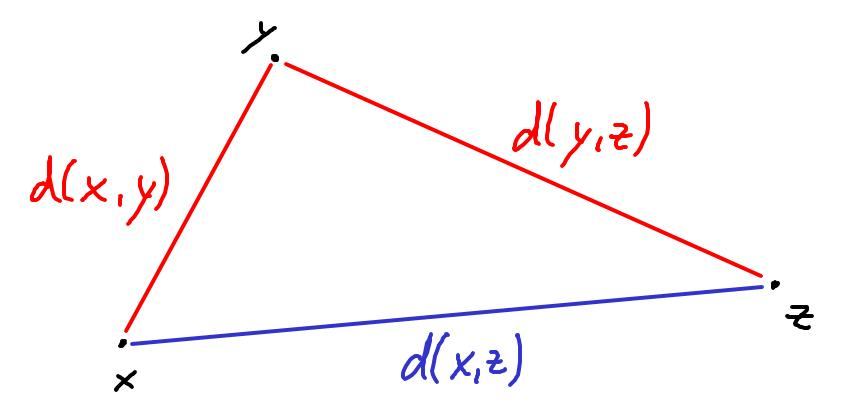
\includegraphics[width=10cm]{./_img/Dreiecksungleichung.jpeg}
        \centering \caption{Dreiecksungleichung: Der direkte Weg $d(x,z)$ ist stets kürzer als der Umweg $d(x,y)+d(y,z)$.}
    \end{figure}
\end{bem}


\begin{bem}
    Manchmal wird die Definitheitseigenschaft auch abgeschwächt, indem anstelle von „$\leftrightarrow$“ nur „$\rightarrow$“ gefordert wird; man spricht dann von einer \emph{Pseudometrik}. Ebenso wird manchmal auch „$\infty$“ als Abstand zugelassen. In jedem Fall aber soll $d$ eine Art „Abstand zwischen Punkten“ bezeichnen.
    
    Die Dreiecksungleichung solltest du dir (mitsamt der bildlichen Erklärung!) einprägen. Bei ihr handelt es sich (auch schon in der Ana1) um das wichtigste Werkzeug zum Abschätzen von Abständen. Versuche, dir die anderen beiden Eigenschaften intuitiv zu merken: Die Symmetrie besagt, dass der Abstand von $x$ zu $y$ gleich dem Abstand von $y$ zu $x$ ist. Die Definitheit impliziert, dass jeder Punkt Abstand Null zu sich selbst hat.
\end{bem}


\begin{de}[Abstand in $\R$]
    Für reelle Zahlen $x,y\in \R$ ist der herkömmliche Abstand definiert durch
        \[ d(x,y) := \vert x -y\vert \]
    Diesbezüglich wird $(\R,d)$ zu einem metrischen Raum, was hier ohne Beweis bleiben soll.\footnote{Einen Beweis findest du z.B. in \cite{AE06}, Satz I.11.4.} Ab sofort wird $\R$ stets mit dieser Abstandsfunktion ausgestattet, ohne dass dies noch einmal ausdrücklich erwähnt würde.
\end{de}


\begin{bsp}
    Beispielsweise ist
        \[ d(5,2)= 3 \qquad\qquad d(-2,5)=7 \qquad\qquad d(3,3)=0 \]
    Für jede reelle Zahl $x\in \R$ ist
        \[ \vert x\vert = \vert x-0\vert = d(x,0) \]
    d.h. der Betrag einer Zahl ist genau ihr Abstand zur Null. 
    \begin{figure}[ht]
        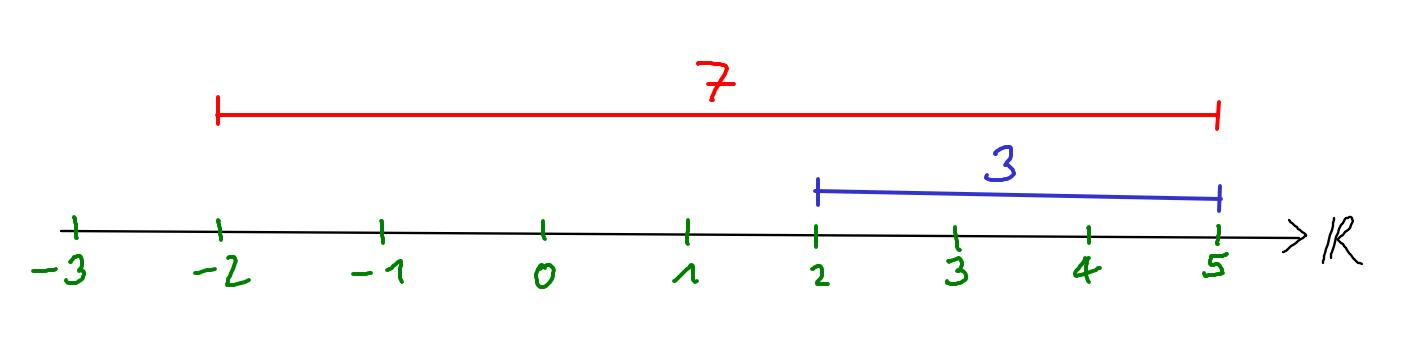
\includegraphics[width=10cm]{./_img/Abstand.jpeg}
        \centering \caption{Abstände auf der reellen Gerade}
    \end{figure}
\end{bsp}


\begin{bsp}[Weitere Metriken] \quad
    \begin{enumerate}
        \item(ebene und räumliche Abstände) In der Ebene $\R^2$, im Raum $\R^3$ und allgemein im Hyperraum $\R^n$ (für ein $n\in \N$) ist der Abstand zweier Punkte gleich der Länge ihrer Verbindungsstrecke. Dies wird in den Analysis-Vorlesungen genauer definiert werden.\footnote{Mehr darüber findest du in \cite{AE06} in Kapitel II.3.} Ich gehe davon aus, dass dir intuitiv klar ist, wie der Abstand zwischen zwei Punkten in der Ebene oder im Raum zu verstehen ist, und werde es ab und zu in einem informellen Sinn nutzen, um mehrdimensionale Beispiele und Illustrationen beisteuern zu können.
        \item(Topologische Datenanalyse) Nicht immer müssen die „Punkte“ eines metrischen Raums eine geometrische Bedeutung besitzen. Beispielsweise wäre ein metrischer Raum $X$ gegeben durch die Menge der Nutzer einer Dating-App, die bei ihrer Anmeldung verschiedene persönliche Vorlieben und Eigenschaften angegeben haben. Für zwei Nutzer $a,b\in X$ könnte dann der „Abstand“ $d(a,b)$ definiert sein als die Anzahl aller Kategorien, in denen $a$ und $b$ verschiedene Präferenzen angegeben haben. Nutzer mit vielen Gemeinsamkeiten wären sich bezüglich dieser Metrik also besonders „nahe“.
    \end{enumerate}
\end{bsp}


\begin{de}[offene Bälle] \label{def:ball} \index{offener Ball}
    Seien $X$ ein metrischer Raum und $a\in X$ ein Punkt. Für $r\in \R_{\ge 0}$ ist der \textbf{offene Ball um $a$ mit Radius $r$} definiert durch
        \[ \bbB_r(a) := \{ x\in X \mid d(a,x)< r\} \]
    $\bbB_r(a)$ ist also die Menge all denjenigen Punkte, deren Abstand zu $a$ strikt kleiner als $r$ ist.
\end{de}


\begin{figure}[ht]
    \begin{minipage}{.48\textwidth}
        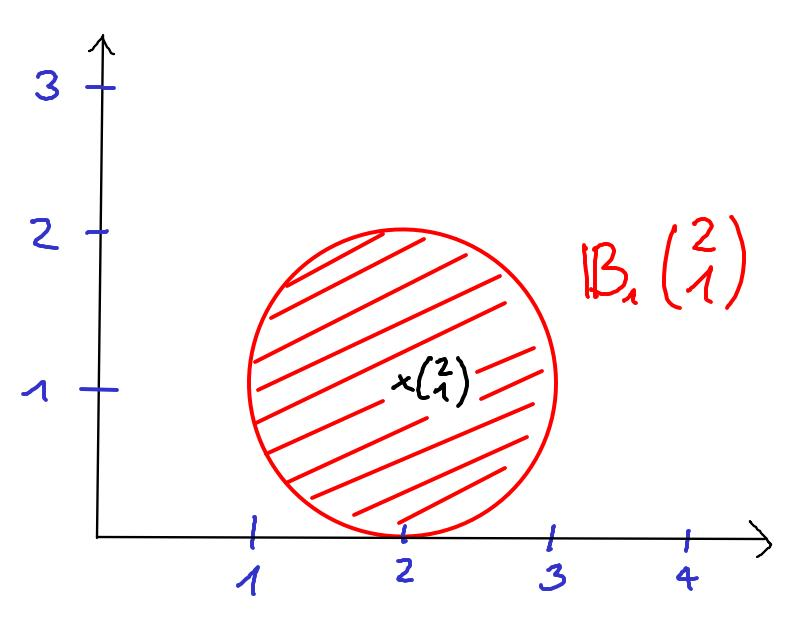
\includegraphics[width=7cm]{./_img/2Dball.jpeg}
        \centering \caption{Der Ball $\bbB_1(2,1)$ im $\R^2$.}
    \end{minipage}
    \quad
    \begin{minipage}{.48\textwidth}
        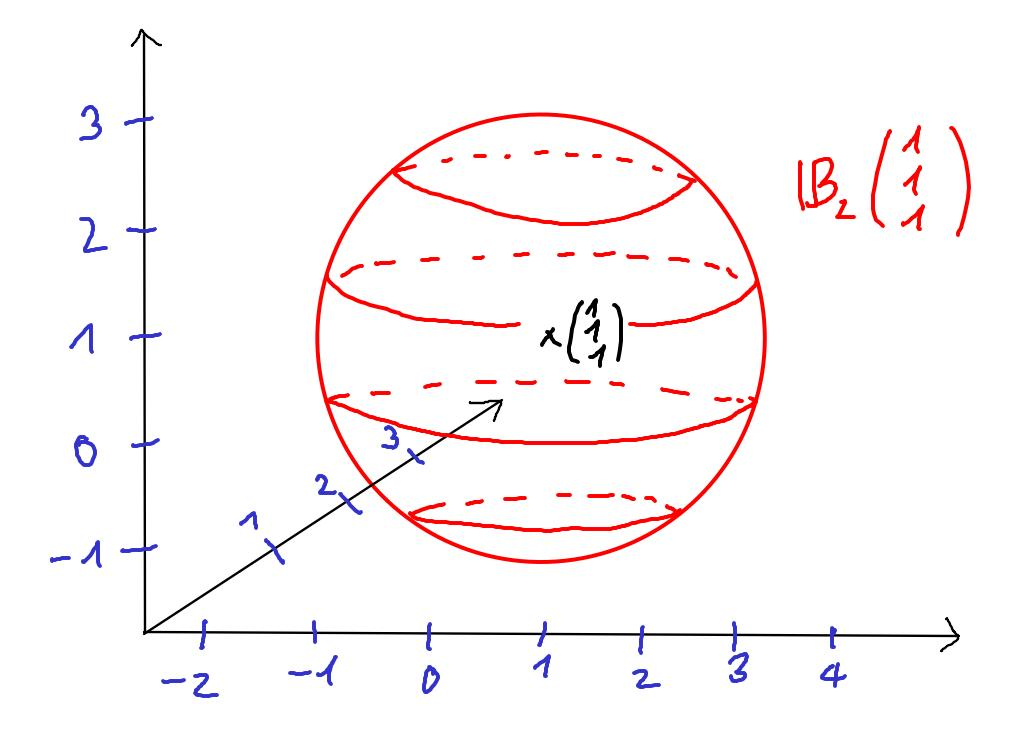
\includegraphics[width=7.5cm]{./_img/3Dball.jpeg}
        \centering \caption{Der Ball $\bbB_2(1,1,1)$ im $\R^3$.}
    \end{minipage}
\end{figure}


\begin{bsp}
    In der Ebene $\R^2$ haben die offenen Bälle die Gestalt einer Kreisscheibe, im Raum $\R^3$ die Gestalt einer Kugel. Beachte, dass die offenen Bälle keinen „Rand“ haben. Denn $\bbB_r(a)$ besteht ja nur aus den Elementen, deren Abstand zu $a$ strikt kleiner als $r$ ist. Diejenigen Elemente, deren Abstand zu $a$ genau gleich $r$ ist (im Zweidimensionalen also genau die Punkte auf dem Kreisrand, im Dreidimensionalen die Punkte auf der Kugeloberfläche), sind nicht in $\bbB_r(a)$ enthalten.
\end{bsp}


\begin{bsp}[offene „Bälle“ in $\R$]
    Betrachte den metrischen Raum $\R$. Für $a=4$ und $r= \frac{3}{2}$ ist
        \[ \bbB_{3/2}(4) = \left\{ x\in \R\mid \vert 4-x\vert <\frac{3}{2} \right\} = \left\{ x\in \R\mid 5/2<x<11/2 \right\} = \left(5/2,11/2\right) \]
    Dies sind genau die Punkte in $\R$, deren Abstand zur $4$ kleiner als $3/2$ ist. Allgemein gilt für reelle Zahlen $a\in \R$ und $r\in \R_{\ge 0}$:
        \[ \bbB_r(a) = (a-r,a+r) \]
    d.h. in $\R$ stimmen die offenen Bälle um $a$ überein mit offenen Intervallen\footnote{zur Definition eines Intervalls siehe \cref{def:intervall}} mit Mittelpunkt $a$.
    
    Dieses Beispiel zeigt, dass die offenen Bälle in allgemeinen metrischen Räumen nicht unbedingt wie „Bälle“ aussehen brauchen.
    \begin{figure}[ht]
        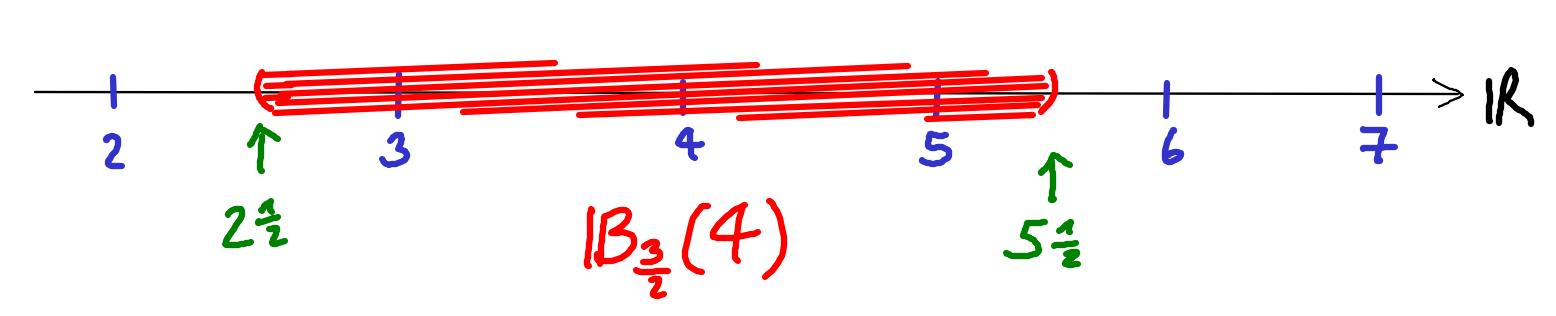
\includegraphics[width=9.5cm]{./_img/1Dball.jpeg}
        \centering \caption{Der offene Ball $\bbB_{3/2}(4)$ in $\R$.}
    \end{figure}
\end{bsp}


\begin{de}[Umgebung in einem metrischen Raum] \label{def:umgebung} \index{Umgebung (Metrische Räume)} \index{innerer Punkt}
    Seien $X$ ein metrischer Raum, $U\subseteq X$ eine Teilmenge und $a\in U$ ein Punkt. $a$ heißt ein \textbf{innerer Punkt von $U$} und $U$ heißt eine \textbf{Umgebung von $a$}, wenn es ein (möglicherweise winzig kleines) $\varepsilon\in \R_{>0}$ gibt mit $\bbB_\varepsilon(a)\subseteq U$.
    \begin{figure}[ht!]
        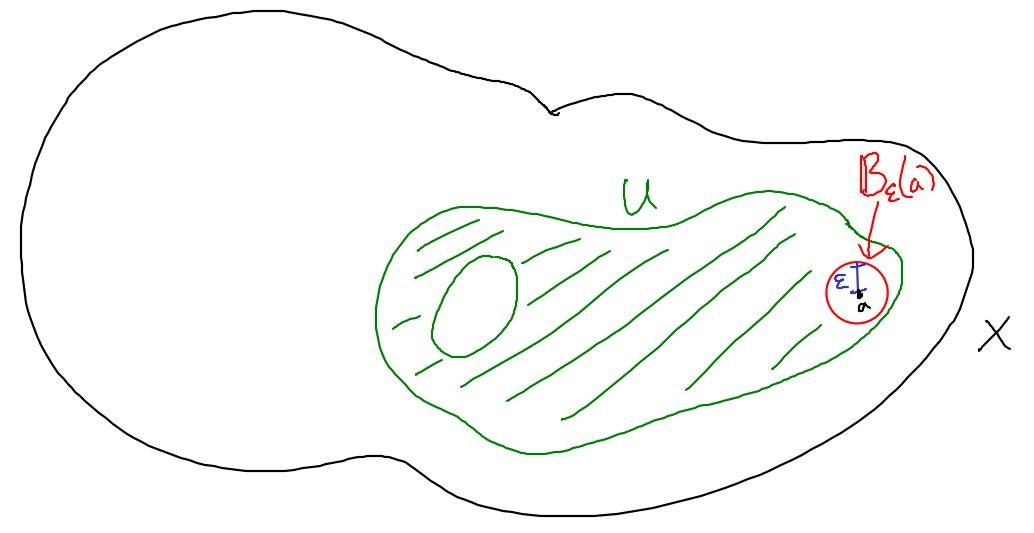
\includegraphics[width=10.5cm]{./_img/Umgebung.jpeg}
        \centering \caption{Im metrischen Raum $X$ ist $U$ eine Umgebung des Punkts $a$, weil sie den $\varepsilon$-Ball $\bbB_\varepsilon(a)$ umfasst.}
    \end{figure}
\end{de}


\begin{bsp}
    Es gilt:
    \begin{enumerate}
        \item Das abgeschlossene Intervall $[0,4]$ ist eine Umgebung der $2$, da $\bbB_1(2)\subseteq [0,4]$.
        \item Dagegen ist $[0,4]$ keine Umgebung der $0$, denn für jedes $\varepsilon\in\R_{>0}$ ist $-\varepsilon/2 \in \bbB_\varepsilon(0)\setminus [0,4]$.
        \item Betrachten wir das Quadrat $Q:=[0,1]\times [0,1]\subseteq \R^2$, so ist $Q$ weder eine Umgebung der Eckpunkte, noch aller weiteren Randpunkte. Denn jeder noch so kleine $\varepsilon$-Ball um einen dieser Randpunkte lugt ja immer ein Stück über den Quadratrand hinaus, ist also nicht vollständig im Quadrat enthalten. Allerdings ist $Q$ eine Umgebung jedes der Punkte im „Inneren“ des Quadrats. Diese letzte Behauptung ist nicht wirklich beweisbar, weil es sich dabei gerade um eine \emph{Definition} des „Inneren“ handelt.
        \item Für einen metrischen Raum $X$ und einen Punkt $a\in X$ ist jeder $\varepsilon$-Ball um $a$ trivialerweise eine Umgebung von $a$, da $\bbB_\varepsilon(a)\subseteq\bbB_\varepsilon(a)$.
    \end{enumerate}
    \begin{figure}[ht!]
        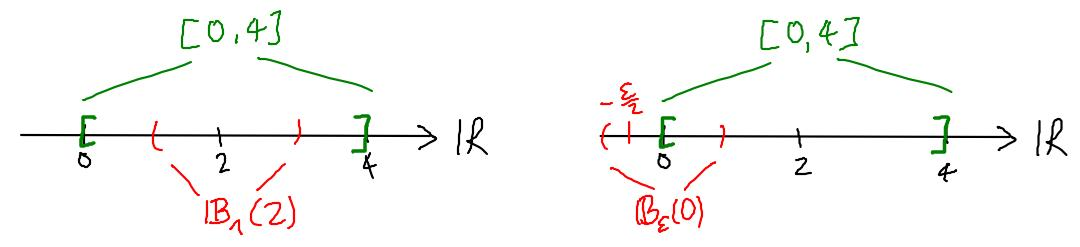
\includegraphics[width=\textwidth]{./_img/Intervallpunkte.jpeg}
        \centering \caption{Das Intervall $[0,4]$ ist eine Umgebung der $2$, aber nicht der $0$.}
        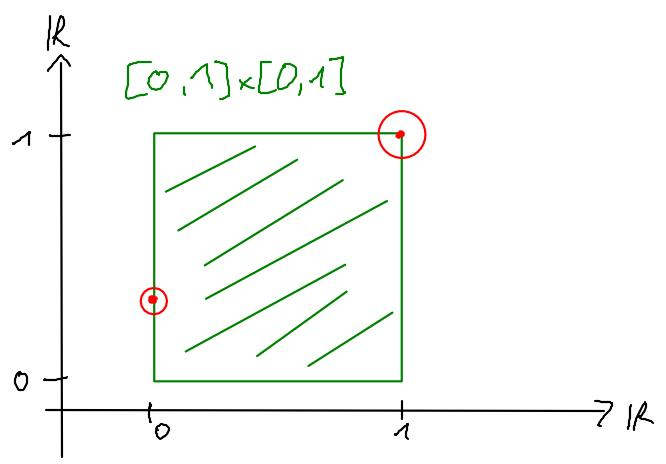
\includegraphics[width=10cm]{./_img/Quadratpunkte.jpeg}
        \centering \caption{Die Randpunkte des Quadrats sind keine inneren Punkte, weil jeder $\varepsilon$-Ball ein Stück weit „über den Rand hinaus reicht“.}
    \end{figure}
\end{bsp}


\begin{bem}[Intuition]
    Die Ansicht, einen „Raum“, wie etwa den euklidischen dreidimensionalen Raum, als eine „Punktmenge“ aufzufassen, ist vergleichsweise jung und trug wesentlich zur Entstehung des Mengenbegriffs, der bei Cantor aus der Untersuchung von Nullstellen gewisser Funktionen $\R \to \R$ erwuchs, bei. Vormals waren der Raum oder die reelle Gerade eher als eine Art „Kontinuum“ verstanden, auf dem zwar einzelne Punkte ausgezeichnet werden können, das aber eine über die Ansammlung von Punkten hinausgehende Qualität der „Kontinuierlichkeit“ besitzt. Auch über die physikalische Realität des Punktbegriffs, eines ausdehnungslosen Orts im Raum oder in der Zeit, lässt sich streiten.\footnote{Mit einer Formalisierung der Konzepte „Nähe“ und „Abweichung“, die unabhängig vom Vorhandensein von Punkten ist, beschäftigt sich die \href{https://en.wikipedia.org/wiki/Pointless_topology}{punktfreie Topologie}, die bislang aber noch keinen Einzug in den mathematischen Mainstream gefunden hat.}
    
    In Physik und Stochastik können meist nur Näherungsbereiche für einen Punkt angegeben werden. Beispielsweise ist die Wahrscheinlichkeit dafür, dass ein Dartspieler exakt die Mitte des Dartboards trifft, exakt $0{,}0\%$, da es sich bei der „Mitte des Boards“ um eine mathematische Idealisierung handelt. Dagegen kann für das Treffen des etwa 1cm breiten Bullseye durchaus eine positive Wahrscheinlichkeit angegeben werden, die bei einem professionellen Spieler wie zum Beispiel Phil ``The Power'' Taylor weit im zweistelligen \%-Bereich liegt.
    
    Beim Bullseye-Feld handelt es sich um eine „Umgebung“ des Board-Mittelpunkts. Per Definition beinhaltet eine Umgebung $U$ eines Punkts $a$ einen $\varepsilon$-Ball. Der Punkt hat also einen gewissen „Puffer“ um sich herum in $U$. Sofern wir den Punkt $a$ nur bis auf eine Genauigkeit in der Größe von $\varepsilon$ verorten können, kann dennoch garantiert werden, dass $U$ den Punkt $a$ enthält.
\end{bem}





\section{Zahlenfolgen}


\begin{bem}[Das Zeichen „$\N$“] \label{natzahlen}
    In diesem Abschnitt (und auch überall sonst in diesem ganzen Skript) wird die Menge der natürlichen Zahlen, sofern die Null eingeschlossen ist, mit „$\N_0$“ bezeichnet und, sofern die Null ausgeschlossen ist, mit „$\N_{\ge 1}$“. In Situationen, in denen es keine Rolle spielt, ob die Null dabei ist oder nicht, schreibe ich einfach nur „$\N$“.
\end{bem}


\begin{de}[Folge] \label{def:folge} \index{Folge}
    Eine \textbf{Folge} ist eine Familie von Objekten $(a_n)_{n\in \N}$, deren Indexmenge die Menge $\N$ der natürlichen Zahlen ist. Ist $n\in \Z$ eine beliebige ganze Zahl, so spricht man manchmmal auch bei Familien, deren Indexmenge $\Z_{\ge n}$ ist, von Folgen. In diesem Fall starten die Indizes nicht bei Eins oder Null, sondern bei $n$. Der Begriff der Folge ist also nicht präzise umrissen, spricht man aber von „der beliebigen Folge $(a_n)$“ so ist damit gemeint, dass die Indexmenge gleich $\N$ (mit oder ohne Null) ist.
    
    Sind $A$ eine Menge und $(a_n)_{n\in \N}$ eine Folge, deren Einträge allesamt in $A$ liegen, so spricht man von einer \emph{Folge von Elementen aus $A$} oder einer „$A$-wertigen Folge“. Nach \cref{def:mengenpotenz} bezeichnet
    \[ A^\N := \{ (a_n)_{n\in \N} \mid \forall n\in \N: a_n\in A \} \]
    die Menge aller Folgen mit Einträgen aus $A$. Im Spezialfall $A=\R$ spricht man von \textbf{reellen Zahlenfolgen} oder auch \textbf{reellwertigen Folgen}. Analog spricht man von rationalen Zahlenfolgen, Folgen ganzer Zahlen oder komplexen Zahlenfolgen, falls es sich um Elemente von $\Q^\N$, $\Z^\N$ oder $\C^\N$ handelt.
\end{de}


\begin{nota}
    Folgen lassen sich sowohl durch eine exakte Angabe definieren, etwa
    \begin{align*}
        (n^2)_{n\in \N_0}
    \end{align*}
    als auch durch eine suggestive Aufzählung der ersten paar Folgenglieder, etwa
        \[ 0,\quad 1,\quad 4,\quad 9,\quad 16,\quad 25,\quad\dots \]
    Die „Definition durch Auflistung“ ist allerdings nicht mathematisch präzise und sollte nur dann benutzt werden, wenn wirklich unmissverständlich klar ist, welche Folge gemeint ist. Würdest du etwa erahnen, dass mit
        \[ 0,\quad 2,\quad 12,\quad 36,\quad 80,\quad 150,\quad 252,\quad 392,\quad \dots\]
    die Zahlenfolge $(n^2\cdot (n+1))_{n\in \N_0}$ gemeint sein soll?
\end{nota}


\begin{bem}[Folge vs. Menge ihrer Einträge]
    Eine Folge $(a_n)_{n\in \N}$ ist nicht mit der Menge ihrer Einträge $\{a_n\mid n\in \N\}$ zu verwechseln.\footnote{vgl. \cref{mengeeinerfamilie}} Beispielsweise sind die beiden Zahlenfolgen
    \begin{align*}
        1,\quad 2,\quad 3,\quad 1,\quad 2,\quad 3,\quad 1,\quad 2,\quad \dots \\
        1,\quad 3,\quad 2,\quad 1,\quad 3,\quad 2,\quad 1,\quad 3,\quad \dots
    \end{align*}
    voneinander verschieden, während die Mengen ihrer Einträge (nämlich nur $1$, $2$ und $3$) übereinstimmen.
\end{bem}


\begin{bsp}
    Beispiele für reelle Zahlenfolgen sind:
    \begin{enumerate}
        \item Die Folge der Primzahlen $2,3,5,7,11,\dots$.
        \item Die Folge der natürlichen Zahlen $0,1,2,3,4,\dots$.
        \item Die „alternierende Folge“ $((-1)^n)_{n\in \N_0}$. Also $1,-1,1,-1,1,-1,1,\dots$.
        \item Die Folge $0,1,-1,2,-2,3,-3,4,\dots$. Es handelt sich um diejenige Folge $(a_n)_{n\in \N_0}$ mit den Einträgen
        \begin{align*}
            a_n := \begin{cases}
                -\frac{n}{2} & n\ \text{ist eine gerade Zahl} \\
                \frac{n+1}{2} & n\ \text{ist eine ungerade Zahl}
            \end{cases} && n \in \N_0
        \end{align*}
        \item Die Folge der Kehrwerte natürlicher Zahlen $(1/n)_{n\in \N_{\ge 1}}$. Das ist  $1,\frac{1}{2},\frac{1}{3},\frac{1}{4},\frac{1}{5},\dots$. Bei dieser Folge gehen die Indizes erst bei Eins los.
        \item Die Folge $\left(\frac{n}{n+1}\right)_{n\in \N_0}$. Also $0,\frac{1}{2},\frac{2}{3},\frac{3}{4},\frac{4}{5},\dots$.
        \item Die „konstante Folge“ $(3)_{n\in \N}$. Also $3,3,3,3,3,\dots$.
        \item Für $q\in \R$ die Folge der $q$-Potenzen $(q^n)_{n\in \N_0}$ Im Fall $q=2$ erhielte man beispielsweise die Folge der Zweierpotenzen $1,2,4,8,16,\dots$.
    \end{enumerate}
    In all diesen Beispielen gehorchen die Folgenglieder einer einfachen Regel. Dies muss aber nicht immer der Fall sein. Eine Folge darf auch völlig chaotisch sein und ihre Einträge brauchen keinem Muster zu gehorchen. Möglichst chaotische Folgen können mit einem Programm zur Berechnung von Zufallszahlen erzeugt werden.
        
    Hier ist noch ein Beispiel für eine Folge, deren Einträge mal keine Zahlen sind:
    \begin{enumerate}[(9)]
        \item Die Folge $(\{1,\dots , n\})_{n\in \N_0}$, deren Einträge die „Anfangsstücke“ von $\N_{\ge 1}$ sind. Also
            \[ \emptyset\ ,\quad \{1\}\ ,\quad \{1,2\}\ ,\quad \{1,2,3\}\ ,\quad \{1,2,3,4\}\ , \quad \dots \]
        Dies ist keine Zahlenfolge, sondern eine Folge von Mengen. Sie besitzt die Eigenschaft, dass für jedes $n\in \N_0$ ihr $n$-ter Eintrag eine Menge ist, die genau $n$-viele Elemente enthält.
    \end{enumerate}
    Eine riesige Datenbank ganzzahliger Zahlenfolgen ist die \href{https://oeis.org/}{On-Line Encyclopedia of Integer Sequences}.
\end{bsp}


\begin{de}[Beschränktheit] \index{beschränkte Folge}
    Eine reelle Zahlenfolge $(a_n)_{n\in \N}\in \R^\N$ heißt \textbf{nach oben beschränkt} bzw. \textbf{nach unten beschränkt}, falls die Menge ihrer Einträge $\{a_n\mid n\in \N\}$ eine nach oben bzw. nach unten beschränkte Teilmenge von $\R$ im Sinne von \cref{def:schranken} ist. Konkret ist die Folge $(a_n)_{n\in \N}$ also genau dann
    \begin{itemize}
        \item \textbf{nach oben beschränkt}, falls es eine Zahl $M\in \R$ gibt derart, dass $a_n\le M$ für alle $n\in \N$ ist. In diesem Fall heißt ein solches $M$ eine \textbf{obere Schranke} für $(a_n)_{n\in \N}$.
        \item \textbf{nach unten beschränkt}, falls es eine Zahl $M\in \R$ gibt mit $a_n\ge M$ für alle $n\in \N$. In diesem Fall heißt ein solches $M$ eine \textbf{untere Schranke} für $(a_n)_{n\in \N}$.
        \item \textbf{beschränkt}, falls sie sowohl nach oben als auch nach unten beschränkt ist.
        \item \textbf{unbeschränkt}, wenn sie nicht beschränkt ist.
    \end{itemize}
\end{de}


\begin{bsp} Es gilt:
    \begin{enumerate}
        \item Die Folge $\left(\frac{n}{n+1}\right)_{n\in \N}$ ist nach unten durch $0$ und nach oben durch $1$ beschränkt.
        \item Die Folge $2,3,5,7,11,\dots$ der Primzahlen ist nach oben unbeschränkt. Dies ist die Aussage des berühmten \emph{Satzes von Euklid} aus \cref{euklid}.
        \item Die alternierende Folge $((-1)^n)_{n\in \N}$ ist beschränkt, da sie nach oben durch $1$ und nach unten durch $-1$ beschränkt ist.
    \end{enumerate}
    Da die Beschränktheit einer Folge allein von der Menge ihrer Einträge abhängt, ist sie unempfindlich gegenüber einer Änderung der Reihenfolge der Folgeneinträge.
\end{bsp}


\begin{de}[Monotonie] \index{Monotonie (von Folgen)} \index{wachsende Folge} \index{fallende Folge}
    Eine Folge reeller Zahlen $(a_n)_{n\in \N}\in \R^\N$ heißt
    \begin{itemize}
        \item \textbf{(monoton) wachsend}, falls für jedes $n\in \N$ gilt, dass $a_{n+1}\ge a_n$.
        \item \textbf{(monoton) fallend}, falls für jedes $n\in \N$ gilt, dass $a_{n+1}\le a_n$.
        \item \textbf{monoton}, falls sie wachsend oder fallend ist.
    \end{itemize}
    Gilt sogar $a_{n+1}>a_n$ für alle $n\in \N$, so sagt man auch, die Folge sei \emph{strikt wachsend}. Ähnlich definiert man \emph{strikt fallend}.
\end{de}


\begin{bsp}
Es gilt:
    \begin{enumerate}
        \item Die alternierende Folge $((-1)^n)_{n\in \N}$ ist nicht monoton, da zum Beispiel $(-1)^3< (-1)^4$ aber auch $(-1)^4>(-1)^5$.
        \item Die Folge $\left(\frac{n}{n+1}\right)_{n\in \N}$ ist strikt wachsend.
        \begin{bew}
            Für jedes $n\in \N$ ist
            \begin{align*}
                \frac{(n+1)}{(n+1)+1} - \frac{n}{n+1} & = \frac{1}{(n+2)(n+1)} >0
            \end{align*}
            sodass $\frac{(n+1)}{(n+1)+1} > \frac{n}{n+1}$ ist. \qed
        \end{bew}
        \item Für $q\in \R_{\ge 1}$ ist die Folge $(q^n)_{n\in \N}$ monoton wachsend.
        \begin{bew}
            Weil für jedes $n\in \N$ gilt:
            \begin{align*}
                q^{n+1} & = q \cdot q^n \\
                & \ge 1 \cdot q^n && (\text{wegen $q\ge 1$ und $q^n>0$})\\
                & = q^n &&&& \qed
            \end{align*}
        \end{bew}
    \end{enumerate}
\end{bsp}


\begin{de}[``eventually''] \label{def:eventually} \index{eventually (Folgenverhalten)}
    Seien $(a_n)_{n\in \N}$ eine Folge und $E$ eine Eigenschaft. Ich sage, die Folge $(a_n)_{n\in \N}$
    \begin{itemize}
        \item[] \textbf{besitzt die Eigenschaft $E$ für hinreichend große $n$}\footnote{Im Englischen ist die Sprechweise ``the sequence \href{https://en.wikipedia.org/wiki/Eventually_(mathematics)}{eventually} satisfies $E$'' üblich. Leider besitzt sie kein etabliertes Pendant im Deutschen.},
    \end{itemize}
    falls es ein $N\in \N$ gibt derart, dass die Folge $a_N,a_{N+1},a_{N+2},\dots$ die Eigenschaft $E$ besitzt. Salopp gesagt: „Es gibt einen Zeitpunkt $N$ derart, dass diejenige Folge, bei der erst zum Zeitpunkt $N$ eingestiegen wird, die Eigenschaft $E$ besitzt.“
\end{de}


\begin{bsp} \label{bsp:eventually} \quad
    \begin{enumerate}
        \item Die Folge
            \[ 0,\quad -1,\quad -2,\quad -1,\quad 0,\quad 1,\quad 2,\quad 3,\quad 4, \quad 5,\dots \]
        ist nicht monoton. Sie könnte aber zu einer strikt wachsenden Folge gemacht werden, ließe man die ersten zwei Folgenglieder weg. Somit ist sie „wachsend für hinreichend große $n$“.
        \item Die alternierende Folge $((-1)^n)_{n\in \N}$ ist dagegen nicht einmal für hinreichend große $n$ wachsend, denn egal wie spät wir auch einsteigen, immer wieder geht es von $-1$ zu $1$ herauf und von $1$ zu $-1$ herunter.
        \item Ist $\varepsilon \in \R_{>0}$ eine (unter Umständen winzig kleine) positive reelle Zahl, so sind die Einträge der Folge $\left(\frac{1}{n}\right)_{n\in \N}$ dennoch für hinreichend große $n$ (um genau zu sein für $n> \frac{1}{\varepsilon}$) kleiner als $\varepsilon$. Mit anderen Worten: Die Brüche $\frac{1}{n}$ werden „für hinreichend große $n$ beliebig klein“.
    \end{enumerate}
\end{bsp}





\section{Folgenkonvergenz}


\begin{bem}[Intuition]
    \begin{figure}[ht]
        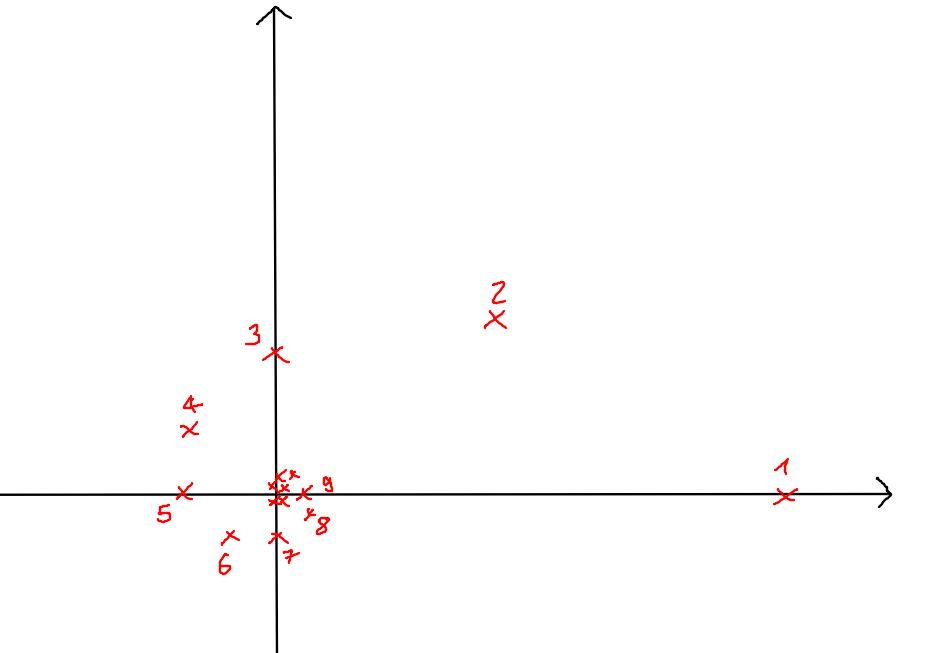
\includegraphics[width=10cm]{./_img/Spirale.jpeg}
        \centering \caption{Eine konvergente Folge von Punkten in der Ebene}
    \end{figure}
    Betrachten wir einmal eine Folge von Punkten in der Ebene, die sich spiralenförmig dem Ursprung annähert. Konkret könnte man
    \begin{align*}
        a_n & := \frac{1}{n}\cdot \begin{pmatrix}
            \cos(n\cdot \pi/4) \\
            \sin(n\cdot \pi/4)
        \end{pmatrix} && n\in \N
    \end{align*}
    definieren, aber das soll gerade keine Rolle spielen.
    
    Du siehst, dass die Folgenglieder dem Koordinatenursprung immer näher kommen, dass sie ihm „für hinreichend große $n$ beliebig nahe kommen“. Genau das heißt Konvergenz.
\end{bem}


\begin{de}[Folgenkonvergenz] \label{def:konvergenz} \index{konvergente Folge} \index{Grenzwert} \index{divergente Folge} \index{Limes}
    Seien $X$ ein metrischer Raum, $(a_n)_{n\in \N}$ eine Folge in $X$ und $a\in X$ ein Punkt. Man sagt, die Folge $(a_n)_{n\in \N}$ \textbf{konvergiert} gegen $a$, falls eine der folgenden beiden äquivalenten Aussagen gilt:
    \begin{enumerate}[(i)]
        \item Für jede (noch so kleine) Umgebung $U$ von $a$ gilt: Für hinreichend große $n$ liegen alle $a_n$'s in $U$.
        \item Für jedes (noch so kleine) $\varepsilon \in \R_{>0}$ gibt es ein $N\in \N$ derart, dass $d(a_n,a)<\varepsilon$ für alle $n\in \N_{\ge N}$. Als Formel:
        \begin{align*}
            \forall\varepsilon\in \R_{>0}\ \exists N\in\N\ \forall n\in \N_{\ge N}:\ d(a_n,a)<\varepsilon
        \end{align*}
    \end{enumerate}
    In diesem Fall heißt $a$ ein \textbf{Grenzwert} oder \textbf{Limes} der Folge $(a_n)_{n\in \N}$. Man schreibt
        \[ \lim_{n\to\infty}a_n=a \qquad\text{oder}\qquad a_n\xrightarrow[n\to \infty]{} a \]
    Eine Folge, die einen Grenzwert besitzt, heißt \textbf{konvergent}. Andernfalls heißt sie \textbf{divergent}.
\end{de}


\begin{bew}[*]
    (i)$\to$(ii): Sei $\varepsilon\in \R_{> 0}$ beliebig. Weil der $\varepsilon$-Ball $\bbB_\varepsilon(a)$ eine Umgebung von $a$ ist, folgt aus (i), dass die $a_n$'s für hinreichend großes $n$ in $\bbB_\varepsilon(a)$ liegen, also dass es ein $N\in \N$ gibt derart, dass $a_n\in \bbB_\varepsilon(a)$ für alle $n\in \N_{\ge N}$. Per Definition des Balles $\bbB_\varepsilon(a)$ ist dies genau die Aussage von (ii). \\[0.5em]
    (ii)$\to$(i): Sei $U\subseteq X$ eine beliebige Umgebung von $a$. Nach \cref{def:umgebung} gibt es dann ein $\varepsilon\in \R_{>0}$ mit $\bbB_\varepsilon(a)\subseteq U$. Nach (ii) gibt es ein $N\in \N$ derart, dass $d(a_n,a)<\varepsilon$ für alle $n\in \N_{\ge N}$, d.h. für hinreichend großes $n$ haben die $a_n$'s einen Abstand von weniger als $\varepsilon$ von $a$. Nach \cref{def:ball} heißt das gerade, dass die $a_n$'s in $\bbB_\varepsilon(a)$ liegen für hinreichend große $n$, wegen $\bbB_\varepsilon(a)\subseteq U$ also auch in $U$. \qed
\end{bew}


\begin{bem}[„Sei $\varepsilon>0$“] \index{Epsilontik}
    Diese Grenzwertdefinition ist vergleichsweise jung: sie stammt aus dem 19. Jahrhundert und wurde durch Cauchy\footnote{\href{https://de.wikipedia.org/wiki/Augustin-Louis_Cauchy}{Augustin-Louis Cauchy (1789 - 1857)}} und Weierstraß\footnote{\href{https://de.wikipedia.org/wiki/Karl_Weierstra\%C3\%9F}{Karl Weierstraß (1815 - 1897)}} populär. Bis dahin herrschte in der Mathematik ein eher „intuitiver“ Umgang mit Grenzwerten vor.
    
    Definition (i) ist prägnant, recht leicht zu merken und geeignet, um manche allgemeine Sätze zu beweisen. Dagegen ist das Logik-Monstrum (ii) diejenige Definition, die relevant wird, wenn du von einer konkreten Zahlenfolge ausrechnen willst, dass sie konvergiert.
    
    In der Analysis hat es sich eingebürgert, in Definitionen und Beweisen jene Abstände, die „beliebig klein“ werden können, mit einem Epsilon $\varepsilon$ zu notieren. Aus diesem Grund spricht man bei Definitionen und Beweisen der Analysis, die exzessiven Gebrauch von $\varepsilon$'s machen, von „Epsilontik“.
\end{bem}


\begin{bsp} \label{bsp:konvergenz}
    Die durch
    \begin{align*}
        a_n &:= \frac{n}{n+1} && n\in \N
    \end{align*}
    definierte reelle Folge $(a_n)_{n\in \N}\in \R^\N$ konvergiert gegen $1$.
\end{bsp}


\begin{figure}[ht]
    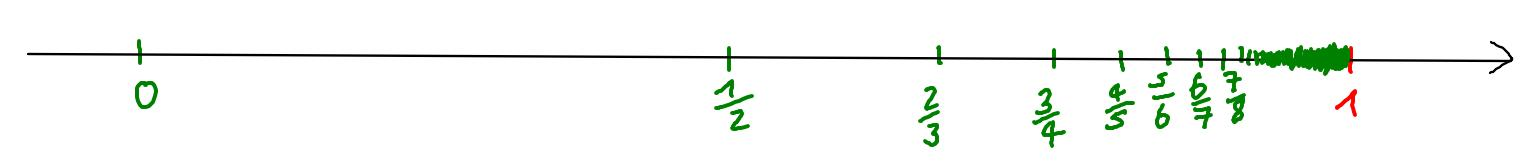
\includegraphics[width=14cm]{./_img/Konvergenzbsp.jpeg}
    \centering \caption{Die Folge $\left(\frac{n}{n+1}\right)_{n\in \N}$ konvergiert gegen $1$.}
\end{figure}


\begin{bem}
    Bevor wir versuchen, für diese Aussage einen Bilderbuchbeweis hinzuschreiben, wollen wir „auf dem Skizzenblatt“ erstmal ein paar Überlegungen anstellen:
    
    Nach \cref{def:konvergenz}(ii) müssen wir für ein beliebiges $\varepsilon \in \R_{>0}$ ein $N\in \N$ finden mit der Eigenschaft, dass für alle $n\in \N_{\ge N}$ gilt:
    \begin{align*}
        \varepsilon &  > d\left(1,\frac{n}{n+1}\right)
    \end{align*}
    Mit ein paar Umformungen ergibt sich:
    \begin{align*}
        d\left(1,\frac{n}{n+1}\right) & = \left| 1-\frac{n}{n+1}\right| \\
        & = \left| \frac{n+1}{n+1} - \frac{n}{n+1} \right| \\
        & = \left| \frac{1}{n+1}\right| \\
        & = \frac{1}{n+1} & (\text{da $n\in \N$})
    \end{align*}
    Die Ungleichung $\varepsilon >d(1,n/(n+1))$ lautet also
        \[ \varepsilon > \frac{1}{n+1} \]
    Mit den Umformungen aus \cref{bsp:ungleichungumstellen} kann dies nach $n$ umgestellt werden:
        \[ n > \frac{1}{\varepsilon} -1  \]
    Wählen wir also für $N$ die nächstgrößere natürliche Zahl oberhalb von $1/\varepsilon$, indem wir $1/\varepsilon$ aufrunden (man könnte für $N$ auch jede weitere Zahl, die größer als $1/\varepsilon -1$ ist, verwenden). Dann sind sowohl $N$ als auch alle $n\in \N_{>N}$ größer als $1/\varepsilon- 1$, sodass die Ungleichung aufgeht.
    
    Damit haben wir die Aufgabe auf dem Schmierblatt gelöst. Im finalen Beweis lassen wir die Überlegungen, die uns zur Wahl von $N$ geführt haben, weg. Dies tritt häufig in Analysis-Beweisen auf: die Beweise unterdrücken den Gedankenprozess, der zu ihrem Auffinden geführt hat und verlaufen genau in die entgegengesetzte Richtung:
\end{bem}


\begin{bew}
    Es sei $\varepsilon \in \R_{>0}$ beliebig. Sei $N\in \N$ irgendeine natürliche Zahl, die größer als $1/\varepsilon$ ist. Für alle $n\in \N_{\ge N}$ gilt dann:
    \begingroup
    \allowdisplaybreaks
    \begin{align*}
        d(1,a_n) & = \left| 1-\frac{n}{n+1}\right| \\
        & = \left| \frac{1}{n+1} \right| \\
        & = \frac{1}{n+1} \\
        & \le \frac{1}{N} & (\text{da $N\le n$})\\
        & < \varepsilon & (\text{da $N> 1/\varepsilon$})
    \end{align*}
    \endgroup
    Somit liegen ab dem $N$-ten Eintrag alle Folgenglieder in $\bbB_\varepsilon(1)$. Da $\varepsilon \in \R_{>0}$ beliebig gewählt war, ist damit bewiesen, dass die $a_n$'s gegen $1$ konvergieren. \qed
\end{bew}


\begin{bem}
    Beachte, dass die Tatsache, ob eine Folge konvergiert oder divergiert, eine reine Eigenschaft des „Langzeitverhaltens“ dieser Folge ist. Die ersten paar Millionen Folgenglieder haben für sich allein keinen Einfluss auf das Konvergenzverhalten, weil die Folge ja ab dem dreimillionsten Eintrag plötzlich eine ganz andere Richtung einschlagen könnte. (Die Folgen, mit denen du es in der Vorlesung zu tun hast, unterliegen aber meist einem einfachen Muster, das spätestens nach ein paar Dutzend Folgengliedern ersichtlich sein sollte.)
\end{bem}


\begin{bsp}[Konstante Folgen konvergieren]
    Seien $X$ ein metrischer Raum und $x \in X$ ein beliebiger Punkt. Dann konvergiert die konstante Folge $(x)_{n\in \N}$ gegen $x$.
        \[ x,x,x,x,\dots \qquad \xrightarrow[n\to \infty]{} x \]
\end{bsp}
    
    
\begin{bew}
    Sei $U$ eine beliebige Umgebung von $x$. Wegen $x\in U$ liegt die konstante Folge $(x)_{n\in \N}$ vollständig in $U$. Weil die Umgebung $U$ beliebig gewählt war, konvergiert die Folge nach \cref{def:konvergenz}(i) also gegen $x$.
\end{bew}


\begin{bem}
    Der Satz lässt sich dahingehend verallgemeinern, dass auch schon jede Folge, die für hinreichend große $n$ konstant gleich $x$ ist, gegen $x$ konvergiert. In diesem Fall liegt die Folge zwar nicht mehr unbedingt vollständig in der Umgebung $U$, aber immer noch für hinreichend große $n$, und dies reicht ja schon aus für das Vorliegen von Konvergenz.
\end{bem}


\begin{vorschau}[* Ordnungstopologie]
    Es ist möglich, Konvergenz reellwertiger Folgen rein ordnungstheoretisch zu definieren. Sind $a\in \R$ und $(a_n)_{n\in \N}$ eine Folge reeller Zahlen, so kann man definieren, dass die $a_n$'s gegen $a$ konvergieren genau dann, wenn für alle $x\in \R_{<a}$ und alle $y\in \R_{>a}$ gilt, dass die $a_n$'s für hinreichend große $n$ allesamt größer als $x$ und kleiner als $y$ sind. Auf dieser Weise lässt sich auch die Konvergenz von Folgen auf der erweiterten Zahlengerade $\bar \R$ definieren. Zum Beispiel gälte dann $\lim_{n\to\infty} n^2=\infty$.
    
    Das dahinterliegende Prinzip heißt \href{https://de.wikipedia.org/wiki/Ordnungstopologie}{Ordnungstopologie} und erlaubt es, die Konzepte „Umgebung“ und „Konvergenz“ in beliebigen totalgeordneten Mengen zu definieren, ohne dass sie mit einer Abstandsfunktion ausgestattet sein müssen. Für viele „Räume“ in der Analysis wie z.B. $\C$ oder der $\R^3$ ist das Konzept des metrischen Raums aber wohl angebrachter.
\end{vorschau}





\section{Analytisches Arbeiten}


\begin{satz}[Rechenregeln für Folgengrenzwerte] \label{konvergenzregeln}
    Seien $(a_n)_{n\in \N},(b_n)_{n\in \N}\in \R^\N$ zwei konvergente Folgen mit $a:=\lim_{n\to\infty}a_n$ und $b:=\lim_{n\to\infty}b_n$. Dann gilt:
    \begin{enumerate}[a)]
        \item $\lim_{n\to\infty}(a_n+b_n)=a+b$
        \item $\lim_{n\to\infty}(\lambda \cdot a_n)=\lambda \cdot a$ für $\lambda\in\R$
        \item $\lim_{n\to\infty}(a_n\cdot b_n)=a\cdot b$.
        \item $\lim_{n\to\infty}\frac{a_n}{b_n} = \frac{a}{b}$, sofern $b\neq 0$ und $b_n\neq 0$ für alle $n\in \N$.
    \end{enumerate}
\end{satz}


\begin{bew}
    Die Aussagen sollen hier ohne Beweis bleiben.\footnote{Beweise findest du etwa in \cite{AE06}, Satz II.2.2 und Satz II.2.4.}. \qed
\end{bew}


\begin{bem}[Komplizierte Objekte in einfache Bausteine zerlegen]
    Sätze wie dieser sind von herausragender Bedeutung für die Analysis. Sofern man einen kleinen Vorrat an Folgen, für die man ihre Konvergenz bewiesen hat, aufgebaut hat, erlauben sie es, Grenzwerte für die kompliziertesten Folgen auszurechnen, ohne dass man für einen Beweis nochmal die $\varepsilon$'s auskramen müsste.
    
    Beispielsweise würde kein routinierter Mathematiker einen $\varepsilon$-Beweis dafür führen, dass die Folge
        \[ \left( 1 + \frac{3n}{n+1} \right)_{n\in \N} \]
    gegen $4$ konvergiert. Sondern er würde schlicht bemerken, dass sich diese Folge zerlegen lässt in
        \[ (1)_{n\in \N} + 3\cdot \left(\frac{n}{n+1}\right)_{n\in \N} \]
    und dann auf die Rechenregeln für $\lim_{n\to\infty}(-)$ verweisen. Denn es ist
        \[ \lim_{n\to \infty} \left( 1+ \frac{3n}{n+1} \right) = \left( \lim_{n\to \infty} 1 \right)+3\cdot \left( \lim_{n\to \infty} \frac{n}{n+1} \right) = 1+3\cdot 1 = 4 \]
    Diese Denkweise kennst du auch aus der Schule: Um beispielsweise die Ableitung der Funktion
    \begin{align*}
        f(x) &= (x^2+3x)\cdot e^x && x\in \R
    \end{align*}
    zu berechnen, würdest du ausnutzen, dass sich diese Funktion aus den Bestandteilen
    \begin{align*}
        g(x)& = x^2 \\
        h(x) & = 3x \\
        q(x) &= e^x && x\in \R
    \end{align*}
    zusammensetzt via
    \begin{align*}
        f(x) & = (g(x)+h(x))\cdot q(x) && x\in \R
    \end{align*}
    Mittels Summen- und Produktregel würdest du schlussfolgern
    \begin{align*}
        f'(x) & = (g'(x)+h'(x))\cdot q(x)  + (g(x)+h(x))\cdot q'(x) \\
        & = (2x+3)\cdot e^x + (x^2+3x)\cdot e^x \\
        & = (x^2+5x+3)\cdot e^x && x\in \R
    \end{align*}
    Die „analytische Methode“, komplexe Funktionen in einfache Bestandteile zu zerlegen, ist auch an der Uni überlebensnotwendig. Kein erfahrener Mathematiker würde, um die Ableitung von $(x^2+3x)\cdot e^x$ zu berechnen, unmittelbar mit der Definition der Ableitung arbeiten und versuchen, den Differenzialquotienten
    \begin{align*}
        f'(x)&:=\lim_{h\to 0} \frac{((x+h)^2+3(x+h))\cdot e^{x+h} - (x^2+3x)\cdot e^{x}}{h} && x\in \R
    \end{align*}
    direkt auszurechnen. \\[0.5em]
    Ein Ziel der Analysis-Vorlesung ist es, dich mit Werkzeugen auszustatten, die das Berechnen von Grenzwerten bequem machen und Epsilontik vermeiden. Versuche in Analysis-Beweisen, die Objekte immer soweit es geht in einfachste Bausteine zu zerlegen und einen $\varepsilon$-Beweis erst wenn gar nichts anderes mehr geht als Ultima Ratio anzusetzen.
\end{bem}


\begin{bsp}
    Schauen wir uns nochmal die Folge $\left(\frac{n}{n+1}\right)_{n\in \N}$ aus \cref{bsp:konvergenz} an. Mithilfe der Regeln aus \cref{konvergenzregeln} ergibt sich
    \begin{align*}
        \lim_{n\to\infty} \frac{n}{n+1} & = \lim_{n\to\infty} \frac{1}{1+\frac{1}{n}} && (\text{Bruch um den Faktor $n$ kürzen}) \\
        & = \frac{1}{\lim_{n\to\infty} \left(1+\frac{1}{n}\right)} && (\text{\cref{konvergenzregeln}d)}) \\
        & = \frac{1}{1+\lim_{n\to\infty} \frac{1}{n}} && (\text{\cref{konvergenzregeln}a)}) \\
        & = \frac{1}{1+0} && (\text{da $\lim_{n\to\infty} 1/n=0$, siehe \cref{bsp:eventually}}) \\
        & = 1
    \end{align*}
    Auf diese Weise können wir den Grenzwert berechnen, ohne mit $\varepsilon$'s arbeiten zu müssen.
\end{bsp}





\clearpage
\section{Aufgabenvorschläge}


\begin{aufg}[Ungleichungen auflösen]
    Seien $x,y\in \R$ zwei reelle Zahlen mit $x>0$ und $0<y<1$. Löst die folgenden Ungleichungen nach der Variablen $x$ auf:
    \begin{align*}
        &\text{a)} & 4x + 3 \quad&\le\quad 7x-6 \\[0.5em]
        &\text{b)} & \frac{x-1}{x+1} \quad&\le\quad y \\[0.5em]
        &\text{c)} & x-1 \quad&\le\quad \frac{xy-1}{x+1} \\[0.5em]
        &\text{d)} & \frac{x-2}{x^2-4} \quad&\le\quad 5 && (\text{vorausgesetzt, dass $x\neq \pm 2$})
    \end{align*}
\end{aufg}


\begin{aufg}[Hausdorffeigenschaft\footnote{\href{https://de.wikipedia.org/wiki/Felix_Hausdorff}{Felix Hausdorff (1868-1942)}}]
    Seien $X$ ein metrischer Raum, $a,b\in X$ zwei verschiedene Punkte und $D:=d(a,b)>0$.
    
    Beweist mithilfe der Dreiecksungleichung, dass $\bbB_{D/2}(a)\cap \bbB_{D/2}(b)=\emptyset$, und verdeutlicht die Situation mit einem Bild.
\end{aufg}


\begin{aufg}[Teilmengen skizzieren]
    Visualisiert die folgenden Teilmengen von $\R$ jeweils durch eine Zeichnung und beurteilt, welche Elemente dieser Mengen jeweils innere Punkte sind:
    \begin{align*}
        &\text{a)} && \bigcup_{k\in \Z} [3k+1,\ 3k+2] \\
        &\text{b)} && \bigcup_{n\in \N} \left[ -n,\ \frac{n}{n+1} \right] \\
        &\text{c)} && \bigcap_{n\in \N_{\ge 1}} \bbB_{1/n}(7) \\
        &\text{d)} && \R\setminus \Q
    \end{align*}
\end{aufg}


\begin{aufg}[Konkrete Folgen]
    Untersucht jede der folgenden Folgen darauf, ob sie (nach oben oder unten) beschränkt, monoton oder monoton für hinreichend große $n$ ist.
    \begin{enumerate}[a)]
        \item Die Folge der Kehrwerte natürlicher Zahlen $(1/n)_{n\in \N_{\ge 1}}$. Also $1,\frac{1}{2},\frac{1}{3},\frac{1}{4},\frac{1}{5},\dots$.
        \item Die Folge $0,1,-1,2,-2,3,-3,4,\dots$.
        \item Die Folge $(n^2-6n)_{n\in \N}$. Also $0,-5,-8,\dots$.
        \item Die Folge $(a_n)_{n\in \N}$, wobei $a_n$ definiert sei als die Quersumme von $n$.
    \end{enumerate}
\end{aufg}

